\section*{Tutorial}
Some definitions from linear algebra, which were repeated in the tutorial.

Linear algebra was originally developed from geometry but has come to be an important foundation in mathematics. To keep things simple we'll restrict ourselves to $\R^n$ although other structures could be used.

\begin{Def}[Vector space] 
A vector space (for our purposes) is a set of points $$\R^n=\{(x_1,x_2,...,x_n)|x_i \in \R\}$$ that is closed under linear combination.
\end{Def}

\begin{Def}[Linear Combination] 
A linear combination $w$ is defined as the sum of all the vectors in a set $V$ multiplied with some scalars $\lambda$.
$$w=\sum_{i \in V}{\lambda_i v_i} \qquad \lambda_i \in \R,v_i\in V$$ 
\end{Def}  

As infinite sets are hard to describe we're looking for a \emph{Basis} $S$. Which is a subset of $\R^n$ such that every vector in $\R^n$ can be represented as a unique linear combination of the elements of $S$.

The vectors in a basis must be \emph{linearly independent}, that is none of them can be written as a linear combination of the others. The standard basis for $\R^n$ is the set of $n$-dimensional unit vectors.

\[\left\{\begin{pmatrix}1\\0\\\vdots\\0\end{pmatrix},\begin{pmatrix}0\\1\\\vdots\\0\end{pmatrix},\ldots,\begin{pmatrix}0\\\vdots\\0\\1\end{pmatrix}\right\}\]


\begin{thm} 
Every basis of a vector space $\R^n$ has the same number of elements, which is $n$. 
\end{thm}

This follows for example from \href{http://en.wikipedia.org/wiki/Steinitz_exchange_lemma}{Steinitz exchange lemma}.

\begin{Def}[Subspace]
 A subspace $V$ of a vector space $\R^n$ is spanned by a subset of the a basis of $R^n$. Examples of a subspace in 2D are all the lines going through the point $(0,0) \in \R^2$.
\end{Def}

To get a notion of angle between vectors we introduce the dot product (in euclidian spaces also called: inner product). It is defined as

\[\langle x,y\rangle  = \sum x_iy_i\]

It is related to the law of cosines in two dimensions ($c^2 = a^2+b^2-2ab\cos \gamma$) like this:

\begin{minipage}[hbt]{0.5\linewidth}
\begin{align*}
\norm{\vec c}^2 &= \norm{\vec a}^2 + \norm{\vec b}^2 -2\norm{\vec a}\norm{\vec b}\cos \gamma\\
\norm{a-b}^2 &= \norm{\vec a}^2 + \norm{\vec b}^2 -2\norm{\vec a}\norm{\vec b}\cos \gamma\\
\norm{a}^2-2\langle a,b\rangle +\norm{b}^2 &= \norm{\vec a}^2 + \norm{\vec b}^2 -2\norm{\vec a}\norm{\vec b}\cos \gamma\\
\frac{\langle a,b\rangle }{\norm{a}\norm{b}} = \cos \gamma
\end{align*}
\end{minipage}
\hfill
\begin{minipage}[hbt]{0.3\linewidth}
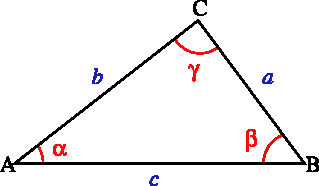
\includegraphics[scale=0.8]{./images/Triangle_with_notations_2.pdf}
\end{minipage}

\bigskip
(Here $\norm{a}$ denotes the norm: $\sqrt{\sum a_i^2} = \sqrt{\langle a,a\rangle }$). Obviously the dot product is 0 if the vectors are orthogonal to each other.

Now that we have defined vector spaces we want to study some linear transformations on them. Since vector spaces are closed under linear combination we'd like to have our transformation preserve that structure.

\begin{Def}[Linear Transformation] A linear transformation is (for our purposes) a mapping $T : \R^n \rightarrow \R^m$ with the following properties:

\begin{enumerate}
\item $T(\lambda w) = \lambda T(w)$
\item $T(v+w) = T(v)+T(w)$
\end{enumerate}
\end{Def}

Prominent examples for linear transformations are rotations and reflections around the origin. Note that if $T(\vec 0)\neq 0$ you automatically know that it's not a linear transformation.

If we use a standard basis for our vector space we can easily represent linear transformations by their effects on the basis. Just map every basis vector to its image and write the results in a matrix. 

\begin{Ex}[Reflection] Suppose we want to reflect every vector in $\R^2$ at the x-axis. If we use the standard base $V = \{(1,0),(0,1)\}$ and compute its reflection $V'=\{(1,0),(0,-1)\}$ we get the matrix

\[R = \begin{pmatrix}
1 & 0 \\
0 & -1
\end{pmatrix}\]

Multiplying a vector with that matrix we get its reflection. Just in case: Matrix multiplication

\[\begin{pmatrix}
a_{11} & a_{12} & \ldots & a_{1n}\\
a_{21} & a_{22} & \ldots & a_{2n}\\
\vdots \\
a_{m1} & a_{m2} & \ldots & a_{mn}
\end{pmatrix} * \begin{pmatrix}x_1\\x_2\\\vdots\\x_n\end{pmatrix} =\begin{pmatrix} \sum_{i=1}^n a_{1i}x_i\\ \sum_{i=1}^n a_{2i}x_i\\\vdots\\\sum_{i=1}^n a_{ni}x_i\end{pmatrix}\]

\end{Ex}

Note that for two transformations $f,g$ and their matrices $A,B$ we have
\[\forall \vec v:\ (f\circ g)(v) = (AB)v\]

\begin{Def}[Kernel of a matrix] 
 The kernel of a matrix $A$ is the set of all vectors $x$ with
$$Ax=0$$
\end{Def}

\begin{Def}[Rank of a matrix]
 The rank of a matrix $A$ is the number of linearly independent columns or rows of $A$. The column and row rank is always the same. In other words the row (column) rank is the dimension of the subspace spanned by the rows of $A$. A matrix $A^{m \times n}$ is said to have a full rank if $rank(A)=min(m,n)$
\end{Def}

If a matrix $A$ has full rank its kernel has dimension 0 and any system of equations $A x=b$ has a unique solution $A^{-1}b$. You can invert such matrices for example by using a Gauss-Jordan elimination.



